% ================================== HEADER ====================================
\documentclass[a4paper, 12pt,]{article}             % sets style/look of many things.
%\documentclass{report}                             % part, chapters, front etc.
% ===================== LANGUAGE ==========================
\usepackage{microtype}               % Subliminal refinements towards typographical perfection
\usepackage[utf8]{inputenc}          % Encoding of input files UTF-8
%\usepackage[norsk]{babel}            % Multilingual support for Plain TeX of LaTeX
\usepackage[T1]{fontenc}             % Standard package for selecting font encodings
\usepackage[scaled]{beramono}        % Font
\usepackage{color}                   % color text
\usepackage{titlesec}                % Select altenative section titles
\usepackage{fancyvrb}                % Sophisticated verbatim text
\usepackage{verbatim}                % Comment environment
\usepackage{listings}                % Formant and render text/code etc.
\usepackage{lipsum}                  % Easy acces to the Lorem lipsum dummy text

% ===================== Header and footers ================
\usepackage{fancyhdr}                % Extensive control of page headers and footers in LaTeX

% ===================== Tabell ============================
\usepackage{enumitem}                % Control layout of itemize, enumerate, description
\usepackage{tabu}                    % Flexible LaTeX tabulars
\usepackage{multicol}                % Multiple columns

% ====================== Math ==============================
\usepackage{mathptmx}                % Use Times as default tect font and provide maths support
% AMS:
\usepackage{amsmath}                 % AMS mathematical facilitis for LaTeX
%\usepackage{amsymb}                  % Math symbols
\usepackage{amsfonts}                % Math fonts
\usepackage{siunitx}                 % SI units
\usepackage{mathtools}               % Different math tools to use with amsmath
\usepackage{bm}                      % Bold symbols in maths mode
\usepackage{gensymb}                 % Generic symbols for both text and math mode

% ====================== Pictures ==========================
\usepackage{placeins}                % Control float placement
\usepackage{epsfig}                  % Include Encapsulated PostScript in LaTeX
\usepackage{graphicx}                % Better figures, graphics, units etc.
\usepackage{subfigure}               % Figures divided into subfigures
\usepackage{epstopdf}                % Convert EPS to PDF using Ghostscript
\usepackage{framed}                  % Framed or shaded regions that can break across pages
\usepackage[font=small]{caption}      % Customising captions in floating environments
\numberwithin{figure}{section}
\usepackage{float}                   % Control of floating environment/figure

% ====================== Div ===============================
\newcommand{\HRule}{\rule{\linewidth}{0.5mm}}
\usepackage[pass]{geometry}          % Flexible and complete interface to document dimensions
\usepackage{parskip}                 % Layout with zero \parindent, non-zero \parskip
\usepackage{lscape}                  % Place selected parts of a document in landscape
\usepackage{exsheets}                % Create exercies sheets and exams
\usepackage{tabto}                   % "Tab" to a measured position in the line
\newcommand\marginsymbol[1][0pt]{%
  \tabto*{0cm}\makebox[\dimexpr-1cm-#1\relax][r]{$\mathbb{P}$}\tabto*{\TabPrevPos}}

\renewcommand{\thesubsection}{\thesection.\alph{subsection}}

% ====================== Hyperlink =========================
\usepackage{hyperref}                % Links in TOC etc.
\hypersetup{
  colorlinks = false,
  pdfborder = {0,0,0},
}
\usepackage[all]{hypcap}             % Better links to floating environment

                           % include preambled pckg.

%For en person

\newcommand\Signature[2]{\par\bigskip
  \setlength\tabcolsep{0pt}
  \begin{tabular}{@{\hspace{.05\textwidth}}>{\centering\arraybackslash}p{.4\textwidth}
      @{\hspace*{.1\textwidth}}>{\centering\arraybackslash}p{.4\textwidth}@{\hspace{.05\textwidth}}}
  \multicolumn{2}{c}{#1, \today} \\[10ex]
  \multicolumn{2}{c}{\rule{.4\textwidth}{0.4pt}} \\
  \multicolumn{2}{c}{#2} \\
  \end{tabular} \par}
  

%For tre personer:
  
%\newcommand\Signature[4]{\par\bigskip
%\setlength\tabcolsep{0pt}
%\begin{tabular}{@{\hspace{.05\textwidth}}>{\centering\arraybackslash}p{.4\textwidth}
%  @{\hspace*{.1\textwidth}}>{\centering\arraybackslash}p{.4\textwidth}@{\hspace{.05\textwidth}}}
%\multicolumn{2}{c}{#1, \today} \\[10ex]
%\multicolumn{2}{c}{\rule{.4\textwidth}{0.4pt}} \\
%\multicolumn{2}{c}{#2} \\[10ex]
%\multicolumn{2}{c}{\rule{.4\textwidth}{0.4pt}} \\
%\multicolumn{2}{c}{#3} \\[10ex]
%\multicolumn{2}{c}{\rule{.4\textwidth}{0.4pt}} \\
%\multicolumn{2}{c}{#4} \\[10ex]
%\end{tabular} \par}


%For flere personer i gruppen (6)

%\newcommand\Signature[7]{\par\bigskip
%  \setlength\tabcolsep{0pt}
%  \begin{tabular}{@{\hspace{.05\textwidth}}>{\centering\arraybackslash}p{.4\textwidth}
%    @{\hspace*{.1\textwidth}}>{\centering\arraybackslash}p{.4\textwidth}@{\hspace{.05\textwidth}}}
%  \multicolumn{2}{c}{#1, \today} \\[10ex]
%  \rule{.4\textwidth}{0.4pt} & \rule{.4\textwidth}{0.4pt} 	\\
%  #2 & #3 \\[10ex]
%   \rule{.4\textwidth}{0.4pt} & \rule{.4\textwidth}{0.4pt} 	\\
%  #4 & #5 \\[10ex]
%  \rule{.4\textwidth}{0.4pt} & \rule{.4\textwidth}{0.4pt} 	\\
%  #6 & #7 \\[10ex]
%  \end{tabular} \par}
                          % include made sign.

\usepackage{csquotes}                               % Context sensitive csquotes
\usepackage{biblatex}                               % Sophisticated Bibliography support
%\usepackage{tabto}
%\usepackage{bm}
%\usepackage{gensymb}
\addbibresource{mybib.bib}

\graphicspath{{figures/},{code/}}

% ================================= OPENING ====================================
% Report:
%\title{
%  \textsc{\LARGE Universitetet i Oslo}\\[0.5cm]
%  \includegraphics[scale=0.3]{uio.png}\\[0.5cm]
%  \textsc{\Large Biologically inspired computing}\\[0.5cm]
%  \textsc{\Large INF4490}\\[0.5cm]
%  \HRule \\[0.4cm]
%  { \huge \bfseries Assignment 2: Multilayer Perceptron}\\[0.4cm]
%  \HRule \\[1.5cm]
%}
%  Assignment:
\title{\vspace{-2cm}INF4490 Mandatory Assignment 2:\\
  Multilayer Perceptron}
\author{Stein Raymond Rudshagen}

\date{\today}

% Removing paragraph indents is sometimes useful:
% \setlength\parindent{0pt}

% Make margins smaler to fit more figures, tables etc on page: (optional)
\addtolength{\oddsidemargin}{-0.8in}
\addtolength{\evensidemargin}{-0.8in}
\addtolength{\textwidth}{1.6in}
\addtolength{\topmargin}{-0.8in}
\addtolength{\textheight}{1.6in}
% ================================================================================

% ================================== DOCUMENT ====================================
\begin{document}
% \pagenumbering{gooble}                                % Remove site number: "gooble"
\renewcommand\marginsymbol[1][0pt]{%
  \tabto*{0cm}\makebox[-1cm][c]{$mathbb{P}$}\tabto*{\TabPrevPos}}

\maketitle
%\pagestyle{empty}
%\cleardoublepage
% =======================================
%\pagestyle{fancy}
%\fancyhead{}
%\fancyfoot[C]{Assignment 2 in course ''INF4490'', Autumn 2016}
%\renewcommand{\headrulewidth}{0pt}
%\renewcommand{\footrulewidth}{1pt}
% =======================================
%\newpage
% ======================================
%\tableofcontents{}
%\clearpage
%\listoffigures
%\clearpage
%\newpage
%\pagenumbering{arabic}
%\pagestyle{fancy}
%\fancyfoot[ol,er]{Assignment 2 in course ''INF4490'', Autumn 2016}
%\fancyfoot[el,or]{Page \thepage}
%\fancyfoot[C]{}
\(\mathbb{P}\) marks the programming exercises, using ``Program language'' to run the programs

  
\section*{Oppgave 1: Formelle språk (2 poeng)}
\begin{enumerate}
  \item La L = {ab, abbb, abc, c} og M = {bba, a}. Hva blir LM? 
  \item Hva blir ML? 
  \item Betrakt språket M*L. Hvilke av følgende uttrykk er i dette språket: a, aa, ab, ac, acc, aacc, 
    aaabbb, $\epsilon$?
  \item Hvilke av disse uttrykkene er i språket (ML)* ?
  \item La N=Ø og P=\{$\epsilon$\}. Hva blir LN og hva blir LP? 
  \end{enumerate}

\textit{Answer:}

\begin{enumerate}
\item LM blir LM = {abba, aba, abbbbba, abbba, abcbba, abca, cbba, ca}
\item LM = ML (med andre ord de er like)
\item M*L = {ac, \ensuremath{\epsilon}}
\item (ML)* = {ac, \ensuremath{\epsilon}}
\item N=Ø (tom mengde) \ensuremath{\rightarrow LN = Ø}, \ensuremath{P=\{\epsilon\}} (tom string) \ensuremath{\rightarrow LP = L}  
\end{enumerate}

\section*{Oppgave 2: Endelige tilstandsmaskiner (4 poeng)}
Denne oppgaven kan gjøres i JFLAP. Du anbefales likevel å løse den med papir og penn først for å få 
eksamenstrening. Så kan du bruke JFLAP til å kontrollere løsningen din.
\begin{enumerate}
  \item Lag en ikke - deterministisk endelig tilstandsmaskin (NFA) som beskriver språket\\  
    L1=L(a*b(a+c)* + ac(b+a)), der alfabetet er A={a, b, c}. (Symbolet + er her disjunksjon)
  \item Lag en deterministisk maskin (DFA) som beskriver det samme språket. 
  \item Lag en tilstandsmaskin som beskriver komplementspråket til L1. 
  \item Hvilke av følgende uttrykk er i L1?
  \end{enumerate}
   
  \clearpage

  \textit{Answer:}
  \begin{enumerate}
  \item  Tegnet det på ark først også tegnet den inn i jflap
\begin{figure}[tbh]
    \centering
    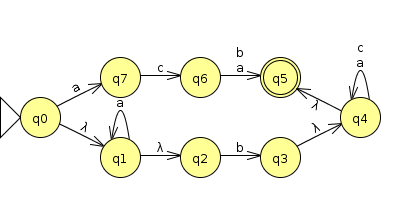
\includegraphics[width=\textwidth, keepaspectratio]{oppg2a.png}
    \caption{Printer ut de regulære uttrykk som tester fire forskjellige strenger hver.}
    \label{fig:awesome_image2}
  \end{figure}
  \item  Lagde først tabell for NFA til DFA, resultatet er på bildet under tabellen.
  % TABLE (TABULAR):
\begin{table}[H]
\centering
  \begin{tabular}{c|c|c c c}
    i & Q & a  & b  & c \\ \hline
    0 & [0,1,2] & [6,1,2] & [3,4,5] & -       \\ 
    1 & [6,1,2] & [1,2]   & [3,2,5] & [7]     \\ 
    2 & [3,4,5] & [4,5]   & -       & [4,5]   \\
    3 & [1,2]   & [1,2]   & [3,4,5] & -       \\
    4 & [7]     & [5]     & [5]     & -       \\
    5 & [4,5]   & [4,5]   & -       & [4,5]   \\
    6 & [5]     & -       & -       & -       \\
  \end{tabular}
  \caption{Tilstandstabell for NFA til DFA}
  \label{tab:oppg2b}
\end{table}

\begin{figure}[tbh]
    \centering
    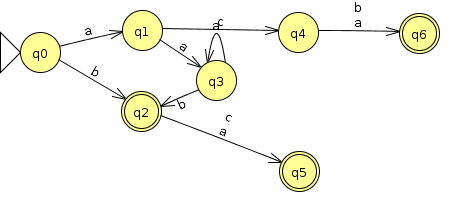
\includegraphics[width=\textwidth, keepaspectratio]{oppg2b.png}
    \caption{Printer ut de regulære uttrykk som tester fire forskjellige strenger hver.}
    \label{fig:awesome_image1}
  \end{figure}

\item Det er den samme tilstandsmaskinen som vist ovenfor.
\item L1 = {'ac(a|b)','ab','aab','aaa*b','b','b(a|c)*'}
\end{enumerate}
  
\section*{Oppgave 3: Regulære uttrykk (4 poeng)}
  Vi skal her bruke hva vi vil kalle "rene" regulære uttrykk.  Det er de vi gikk gjennom på forelesningen 
bygget opp ved 
% TABLE (TABULAR):
\begin{table}[H]
\centering
  \begin{tabular}{l l}
    Regulære uttrykk           & Beskriver språket           \\ \hline
    Ø                          & L(Ø) = Ø                    \\ 
    $\epsilon$                   & L($\epsilon$) = \{$\epsilon$\}  \\ 
    a, for alle a $\epsilon$ A   & L(a) = \{a\}                \\
    Hvis R og S er regulære uttrykk: & \\ \hline
    (R+S) & L(R+S)=L(R)$\cup$L(S) \\
    (R T) & L(R T) = L(R)L(T) \\
    (R*) & L(R*) = L(R)* \\
  \end{tabular}
  \caption{Caption}
  \label{tab:my_label}
\end{table}

La alfabetet A = \{a, b, c\}. Lag regulære uttrykk for følgende språk
\begin{enumerate}
  \item Ord som inneholder minst tre b-er på rad.
  \item Ord som ikke inneholder mer enn to b-er på rad.
  \item Ord hvor antall b-er er delelig med 3 eller antall a-er er delelig med 2 (eller begge deler)
\end{enumerate}

\textit{Answer:}

\begin{enumerate}
  \item (a+b+c)*bbb(a+b+c)*
  \item (a+c)*((ba+bba+bc+bbc)(a+c)*)*(b+bb)
  \item (((a+c)*b(a+c)*b(a+c)*b(a+c)*)*+((b+c)*a(b+c)*a(b+c)*)*)
\end{enumerate}

\section*{Oppgave 4: Regulære uttrykk i Python (2 poeng)}

Test løsningene dine fra oppgave 3 i Python. Dvs. for hver av de tre oppgavene, Kan jeg gjøre denne uten tekstfilen ?

\begin{enumerate}
\item Skriv det regulære uttrykket som et Python-regulært uttrykk! 
\item Lag to eksempler på strenger som skal være i språket og to som ikkje skal være det! 
\item Test uttrykket ditt for de fire strengene! 
\end{enumerate}


\textit{Answer:}

\begin{figure}[tbh]
    \centering
    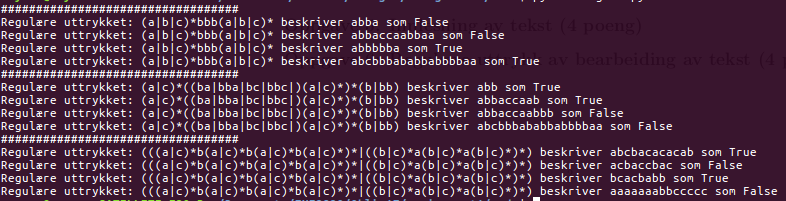
\includegraphics[width=\textwidth, keepaspectratio]{testrun.png}
    \caption{Printer ut de regulære uttrykk som tester fire forskjellige strenger hver.}
    \label{fig:awesome_image}
  \end{figure}

\section*{Oppgave 5: Innlesning av tekst (4 poeng)}

\begin{enumerate}
\item  Les den inn i en interaktiv Python-sesjon som en streng. Kall den "pyt$\_$raw". Oppskriften finner du i 
seksjon 3.1 i NLTK-boka, underavsnitt "Reading local files". Hvis du ser noe rusk i teksten, så rens den. 
\item Når vi videre skal arbeide med en tekst, kan det være en fordel å dele den opp i en liste av ord, der 
hvert ord er en streng. Den enkleste måten å gjøre dette på er ved å bruke split i python. 
>>> pyt$\_$words1 = pyt$\_$raw.split() 
NLTK gir oss også et annet alternativ: 
>>> pyt$\_$words2 = nltk.word$\_$tokenize(pyt$\_$raw) 
Hva blir forskjellen på de to? Ser du fordeler ved å bruke word$\_$tokenize? (Obs! NLTKs word$\_$tokenize 
er optimalisert for engelsk og kan gi noen rare resultat for norsk.) 
\item Et ord som *jeg* er det samme om det står først i en setning og skrives *Jeg*. Tilsvarende for andre 
ord. For en del anvendelser er det derfor en fordel å gjøre om teksten til bare små bokstaver før vi 
går videre. Gjør om alle ordene i pyt$\_$words2 til små bokstaver, og kall resultatet pyt$\_$low. 
\item Plukk ut alle ordforekomstene i pyt$\_$low som inneholder en av de norske bokstavene æ, ø, å. Hvor 
mange slike ordforekomster er det? 
\item  Vi er nå interessert i hvor mange forskjellige ord det er i teksten som inneholder en av de norske 
bokstavene. Plukk ut de unike forekomstene. Hvor mange er det? 
\item Vi skal nå skrive de unike forekomstene til en fil. Når vi skal skrive noe til en fil, kan vi åpne fila ved 
>>> f=open(<filnavn>, 'w') 
Vi kan skrive til fila ved å bruke 
>>> f=write(<det vi vil skrive>) 
Og til slutt lukke fila ved  
>>> f.close() 
 
Skriv de unike forekomstene av ord som inneholder æ, ø eller å til en fil kalt norske.txt, ett ord på 
hver linje.
\end{enumerate}

\textit{Answer:}

\begin{enumerate}
\item Fant ingen rusk, men lest over teksten. Antar pga navnet *raw* så menes det at vi skal lese inn fila og avventer til videre bearbeiding
\item Forskjellen på .split() og nltk_tokenize er at fil.split() spitter ordene default ved whitespace. nltk_tokenize bruker Penn Treebank Tokenizer som skiller ord ved hjelp av regulære uttrykk. Den kan derfor skille ut punktum og comma. Demonstrert nedenfor:

\begin{figure}[tbh]
    \centering
    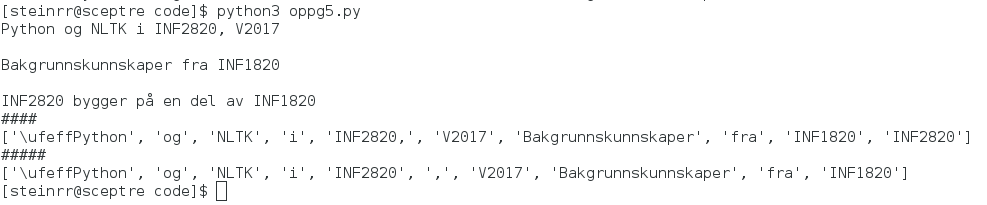
\includegraphics[width=\textwidth, keepaspectratio]{oppg5b.png}
    \caption{Printer ut de regulære uttrykk som tester fire forskjellige strenger hver.}
    \label{fig:awesome_image3}
  \end{figure}
\item 

\section*{Oppgave 6: Regulære uttrykk av bearbeiding av tekst (4 poeng)}



\end{document}
% ==============================================================================
